\documentclass[12pt,a4paper]{article}
\usepackage[margin=2.5cm,left=2cm,includefoot]{geometry}
\usepackage{hyperref}
\usepackage{array}
\usepackage{enumitem}
\usepackage{graphicx}
\usepackage[section]{placeins}
\usepackage{titlesec}

\setlength{\parindent}{0em}

\graphicspath{{Images/}}

\usepackage{fancyhdr}
\pagestyle{fancy}

\rhead{COS 301}
\lhead{Team ProCoder}
\fancyfoot{}
\fancyfoot[R]{Page \thepage}

\renewcommand{\headrulewidth}{2pt}
\renewcommand{\footrulewidth}{1pt}

\begin{document}

\begin{titlepage}
    \begin{center}
        \begin{figure}[t]
            \centering
            
\includegraphics[width=350px]{logo.PNG}
        \end{figure}
        
        \textsc{\LARGE COS301 Final Project \newline \newline Tender Document\\[0.5cm] High Level Description}
        
        \textbf{\newline Team ProCoder} \\
        \begin{flushright} \large
        Bongani Tshela \emph{u14134790} \newline
        Minal Pramlall \emph{u13288157} \newline
        Mandla Mhlongo \emph{u29630135} \newline
        Harris Leshaba \emph{u15312144} \newline
        \end{flushright}
    \vfill
    
    Team ProCoder Github: \href{https://github.com/ProBlack95/COS301-Final-Project}{Github} page.//
    \url{https://github.com/ProBlack95/COS301-Final-Project}
    
    \vfill
    {\large Date:}
    \\
    {\large \today}
    \end{center}
\end{titlepage}

\tableofcontents
\newpage

\section{High Level Description}
This system will be using a behavioral detection method, based on the specification that it will monitor activities and diagnose whether irregular behavior is due to infection.

\begin{figure}
    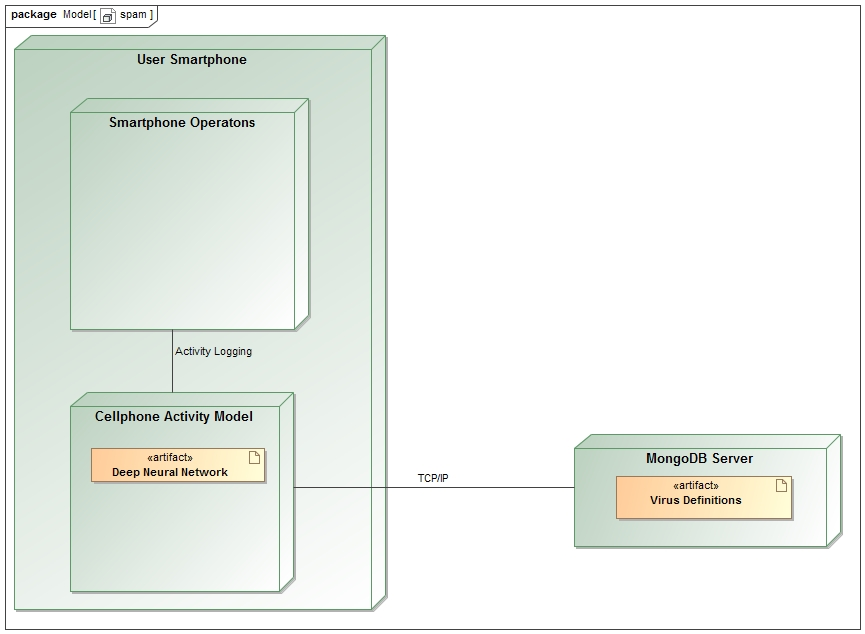
\includegraphics[width=\linewidth]{Images/spam.jpg}
    \caption{Deployment Diagram}
\end{figure}

\section{Development Methodology}
In this system we will deploy a Deep Neural Network to learn from observational data and to distinguish irregular behavior. And, if needed, An object database such as MongoDB, will be employed to keep track of possible virus definitions or behaviours.

\section{Team Skills}
Our team consists of 5 individuals in the final year of our BSc Computer Science or Information Technology degrees, we all have similar skillsets with relation to coding software engineering. The project will be divided up into segments with whichever member feels they will produce the best final product in, then in the final phase, all members will come together and consolidate the system to make sure it meets with the client's expectations.

\end{document}
